\documentclass{article}
\usepackage[utf8]{inputenc}
\usepackage[T2A]{fontenc}
\usepackage{mathtools}
\usepackage{listings}
\usepackage{xcolor}

% \usepackage[dvips]{graphicx}
% \graphicspath{{noiseimages/}}

\definecolor{codegreen}{rgb}{0,0.6,0}
\definecolor{codegray}{rgb}{0.5,0.5,0.5}
\definecolor{codepurple}{rgb}{0.58,0,0.82}
\definecolor{backcolour}{rgb}{0.95,0.95,0.92}

\lstdefinestyle{mystyle}{
    backgroundcolor=\color{backcolour},   
    commentstyle=\color{codegreen},
    keywordstyle=\color{magenta},
    numberstyle=\tiny\color{codegray},
    stringstyle=\color{codepurple},
    basicstyle=\ttfamily\footnotesize,
    breakatwhitespace=false,         
    breaklines=true,                 
    captionpos=b,                    
    keepspaces=true,                 
    numbers=left,                    
    numbersep=5pt,                  
    showspaces=false,                
    showstringspaces=false,
    showtabs=false,                  
    tabsize=2
}

\lstset{style=mystyle}


\title{Исследование практического задания по курсу "Распределенные системы"}
\author{Дмитрий Стамплевский, 421 группа}
\date{}
\begin{document}

\maketitle
\section{Первое задание.}

\subsection{Описание задачи.}
Все 64 процесса, находящихся на разных ЭВМ сети, одновременно выдали запрос на вход в критическую секцию.
Реализовать программу, использующую широковещательный маркерный алгоритм для прохождения всеми процессами критических секций.
Критическая секция:
\begin{verbatim}
    <проверка наличия файла “critical.txt”>;
    if (<файл “critical.txt” существует>) {
        <сообщение об ошибке>;
        <завершение работы программы>;
    } else {
        <создание файла “critical.txt”>;
        Sleep (<случайное время>);
        <уничтожение файла “critical.txt”>;
    }
\end{verbatim}
Для межпроцессорных взаимодействий использовать средства MPI.
Получить временную оценку работы алгоритма. Оценить сколько времени потребуется для прохождения всеми критических секций, если маркером владеет нулевой процесс. Время старта равно 100, время передачи байта равно 1 (Ts=100,Tb=1). Процессорные операции, включая чтение из памяти и запись в память, считаются бесконечно быстрыми.

\subsection{Описание алгоритма.}
Широковещательный алгоритм (он же -- алгоритм Судзуки-Касами) для реализации прохождения всеми процессами критической секции.\\
Есть маркер -- некая структура, содержащая очередь запросов и массив $LN[1...N]$ номеров последних удовлетворенных запросов. У каждого процесса есть свой массив номеров запросов всех процессов: $RN_i$ для процесса с номером $i$.\\
Опишем основные этапы работы алгоритма.
\begin{itemize}

    \item Вход в критическую секцию
        \begin{enumerate}
            \item Если у процесса $i$ нет маркера, он увеличивает $RN_i[i]$ на единицу и посылает другим процессом сообщение "запрос" с номером процесса $i$ и номером запроса $Sn = RN_i[i]$.
            \item Если у процесса есть маркер, он выполняет критическую секцию.
        \end{enumerate}
        
    \item Прием "запроса".\\
    Если процесс $i$ получил сообщение с запросом от процесса $k$, он обновляет свой массив $RN_i$: устанваливает $RN_i[k] = max(RN_i[k], Sn)$. Если у $i$ есть свободный маркер, он посылает его $k$, но при условии, что запрос не устарел, то есть $RN_i[k] = LN[k] + 1$.
    
    \item Выход из критической секции.\\
    Пусть из критической секции выходит процесс $i$, значит маркер в данный момент находится у него.
        \begin{enumerate}
            \item Установить $LN[i] = RN_i[i]$.
            \item $\forall j: RN_i[j] = LN[j] + 1$, такого что $j$ нет в очереди запросов маркера, добавить его в конец очереди.
            \item Если после этого очередь маркера не пуста, удалить из нее первый элемент и переслать ему маркер.
        \end{enumerate}
\end{itemize}

\subsection{Временная оценка алгоритма.}
Для оценки времени работы алгоритма нужно оценить число передач и время их выполнения. Время выполнения передачи = время старта + время на передачу данных. То есть на N байт нужно $T_N = T_s + N * T_b$. Для передачи запроса нужно передать $S_n$ и номер процесса, то есть $100 + 2 * 4 * 1 = 108$ единиц времени (е.в), так как передаются int-ы размером в 4 байта.\\ \textit{В программной реализации номер процесса передается неявно, в status: status.MPI\_Source. Но оценивать работу программы с учетом особенностей MPI значительно сложнее, чем просто сложность алгоритма.}
Оценим размер маркера: минимум по 64 int для LN и 64 для очереди (каждый процесс проходит КС 1 раз). То есть на передачу маркера нужно $100 + 2 * 64 * 4 = 612$ е.в.\\
В описании задания есть один спорный момент, который нужно каким-либо образом решить перед составлением оценки. Критическая секция может работать произвольное время и никаких ограничений на это время не задано. Плюс оценка основана скорее на моей реализации программы. Это отражается в описании порядка работы разных этапов, использовании блокирующих операций.\\
Процесс 0 начал критическую секцию. Выполняет ее какое-то время. Остальные 63 процесса увеличивают номера своих запросов ($RN_i[i]$) на 1 и посылают широковещательные сообщения с этими новыми номерами. То есть с единицами, так как это самое начало работы.\\
Процесс 0 завершает критическую секцию. Теперь он может принять сообщения, полученные от других процессов (запросы). Использовались блокирующие операции, так что он принимает 63 сообщения с $Sn$. Затем он модифицирует маркер, меняет очередь запросов и пересылает маркер первому в очереди процессу. Не ограничивая общности можем сказать, что это будет процесс 1(хотя это в общем случае не совсем определено). Прием маркера процессом 1 и оптравка его процессом 0 происходят одновременно. Время модификации маркера не учитывается. Затем процесс 1 делает то же самое. Затем следующий. В сумме получим следующее время работы: $T_{work} = \sum\limits_{i=0}^{63} T_cs + 63 * T_{Sn} + T_m$, $T_{Sn}$ -- время отправки/приема $Sn$, $T_m$ -- время отправки/приема маркера. То есть $T_{work} = \sum\limits_{i=0}^{63} T_{cs} + 63 * 108 + 612 = T_{cs_{sum}} + 474624$

\subsection{Запуск программы.}
Для запуска первой программы нужно выполнить следубщие действия:
\begin{enumerate}
    \item Перейти в папку с программой
    \item Запустить скрипт командой "./start.sh" или ввести команды вручную:
    \begin{lstlisting}
        mpicc main.c -o task_1.out
        mpirun -np 4 task_1.out
    \end{lstlisting}
\end{enumerate}
Вместо 4 можно указать нужное число процессов. Код программы представлен в конце отчета: \ref{code_1}.

\subsection{Примеры работы программы}
\textit{Здесь представлены результаты запуска на 3 процессах. На 4 и более вывода слишком много и он не помещается на экране}\\
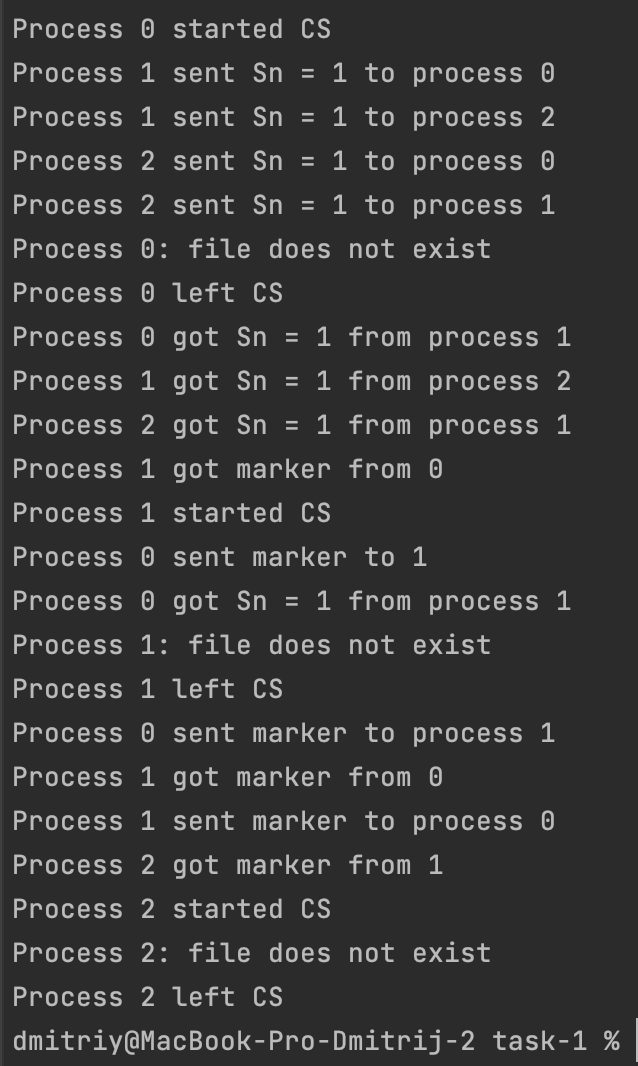
\includegraphics[width=1\linewidth]{task_1_3.png}

\subsection{Выводы.}
Был реализован широковещательный маркерный алгоритм с использованием MPI. Была дана теоретическая оценка времени работы алгоритма для 64 процессов для случая, когда все процессы хотят одноврменно войти в критическую секцию, причем оценка легко адаптируема для любого числа процессов.

\section{Второе задание.}

\subsection{Описание задачи.}
Доработать MPI-программу, реализованную в рамках курса “Суперкомпьютеры и параллельная обработка данных”:
Задание 89. Реализовать параллельное вычисление собственного интеграла методом Симпсона.\\
Добавить контрольные точки для продолжения работы программы в случае сбоя. Реализовать один из 3-х сценариев работы после сбоя: 
\begin{enumerate}
    \item продолжить работу программы только на “исправных” процессах;
    \item вместо процессов, вышедших из строя, создать новые MPI-процессы, которые необходимо использовать для продолжения расчетов;
    \item при запуске программы на счет сразу запустить некоторое дополнительное количество MPI-процессов, которые использовать в случае сбоя.
\end{enumerate}
Был выбран второй вариант: "вместо процессов, вышедших из строя, создать новые MPI-процессы, которые необходимо использовать для продолжения расчетов".

\subsection{Детали реализации.}
В программе для вычисления интеграла не так много мест, где можно использовать контрольные точки. Тем более цель была доработать старую программу, а не переписать ее с нуля. Поэтому был выбран следующий подход к задаче:
\begin{itemize}
    \item Процесс может "сломаться" с некой вероятностью.
    \item Если это происходит, процессы пересоздаются и интеграл вычисляется заново.
    \item Все это происходит в цикле.
\end{itemize}
При таком подходе не приходится хранить лишние данные, но зато при очень большом числе процессов и большой вероятности поломки алгоритм может работать долго. Для таких ситуаций можно создавать массив с результатами работы процессов и не перезапускать все, а считать только случаи ошибок.\\
% Программа частично основана на примерах University of Tennessee Research Foundation, которые приводились в курсе в качестве примеров по обработке ошибок.

\subsection{Запуск программы.}
\begin{enumerate}
    \item Перейти в папку с программой
    \item Выполнить команду source dockervars.sh
    \item Выполнить команду make
    \item Запустить программу: mpirun -np 10 --with-ft ulfm ./task\_2  
\end{enumerate}
Вместо 10 можно указать нужное число процессов. Для запусков после первого необходимо запускать только последнюю команду.
Код программы в конце отчета: \ref{code_2}.

\subsection{Пример работы программы.}
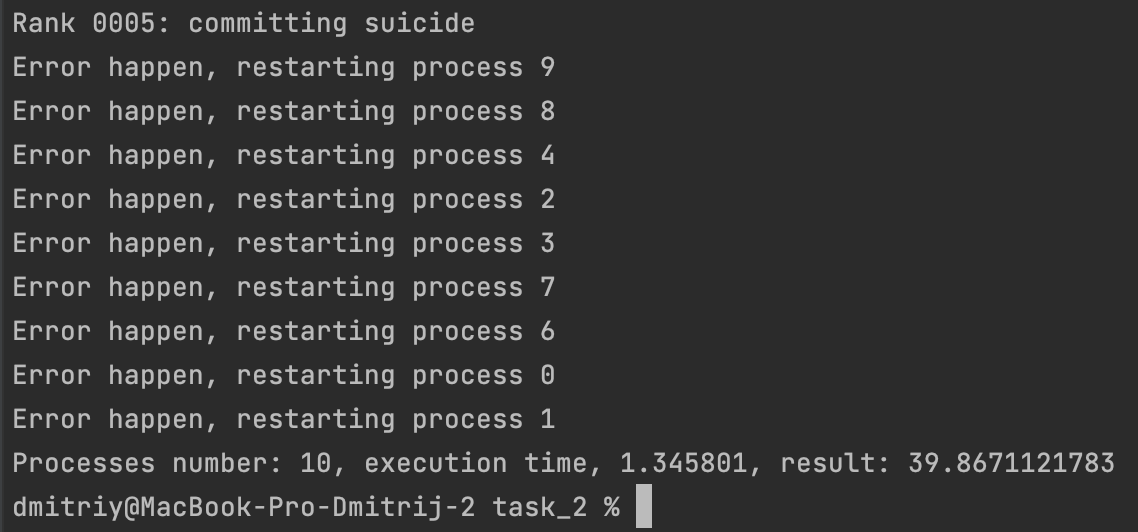
\includegraphics[width=1\linewidth]{task_2_10.png}

\subsection{Выводы.}
Программа для вычисления интеграла методом Симпсона была модернизирована для большей устойчивости. Теперь в случае ошибки в каком-то из процессов (ошибки, при которой вычисления не были завершены) программа может продолжать работу, пересоздавая процессы и заново вычисляя интеграл.

\section{Код первой задачи}\label{code_1}
\lstinputlisting[language=Octave]{task_1.cpp}

\section{Код второй задачи}\label{code_2}
\lstinputlisting[language=Octave]{task_2.cpp}

\end{document}